\documentclass{article}
\usepackage[T1]{fontenc}
\usepackage{lmodern}
\usepackage{graphicx}
\usepackage{amsmath,amssymb}
\usepackage[a4paper,margin=2cm]{geometry}
\usepackage[absolute,overlay]{textpos}
\setlength{\TPHorizModule}{1mm}
\setlength{\TPVertModule}{1mm}
\usepackage[indonesian]{babel}
\usepackage{hyperref}
\setlength{\emergencystretch}{2em}
% unit: Halaman 46

\begin{document}

% === Halaman 46 (llm) ===

\section*{Pseudo-random generation algorithm (PRGA)}

\vspace{64.15mm}

\begin{itemize}
    \item PRGA membangkitkan kunci-alir (\textit{keystream}) dengan cara mengambil nilai $S[i]$ dan $S[j]$, mempertukarkannya, lalu menjumlahkan keduanya dalam modulus 256.
    \item Kunci alir tersebut kemudian di-XOR-kan dengan sebuah karakter plainteks.
\end{itemize}

\vspace{10mm}

\begin{verbatim}
i <- 0
j <- 0
for idx <- 0 to Length(P) - 1 do
    i <- (i + 1) mod 256
    j <- (j + S[i]) mod 256
    swap(S[i], S[j])    {* Pertukarkan nilai S[i] dan S[j] *}
    t <- (S[i] + S[j]) mod 256
    u <- S[t]           (* keystream *)
    c <- u XOR P[idx]   { enkripsi }
end
\end{verbatim}

% deskripsi: Diagram ilustrasi proses PRGA yang menunjukkan array S dengan indeks i, j, dan t, serta operasi swap dan penjumlahan modulo 256.
% bbox normalisasi: [0.5110, 0.3690, 0.9780, 0.5850]
\begin{textblock*}{98.07mm}(107.31mm,109.59mm)
\noindent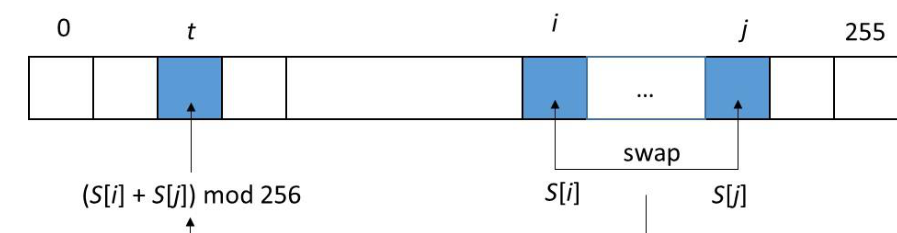
\includegraphics[width=98.07mm,height=64.15mm]{../../images/llm/page_046_img_01.png}%
\end{textblock*}

\end{document}
